\section{Implementation}
\label{sec.implementation}
\noindent The first step towards establishing the technologies which are most
suited for this project, was to draw a high level architecture of the system. As
the system is a lot about user interaction (i.e. presentation layer) and can get
rather big and complex, we decided to go for a concrete separation between the
\emph{domain~logic} and the \emph{user~interface}; the way to go in order to
achieving this separation in a web application is by relying on the
\emph{n-Tier} architectural pattern. As we also need a \emph{persistent~storage}
which should also be separated by the \emph{domain-login} and
\emph{user-interface}, we notice that our application is structured into
\emph{three layers}. Hence, we are dealing with a system leveraging the
\emph{3-Tier} architectural pattern, depicted in Figure \ref{fig.setup}.
\begin{figure}[H] 
	\centering
	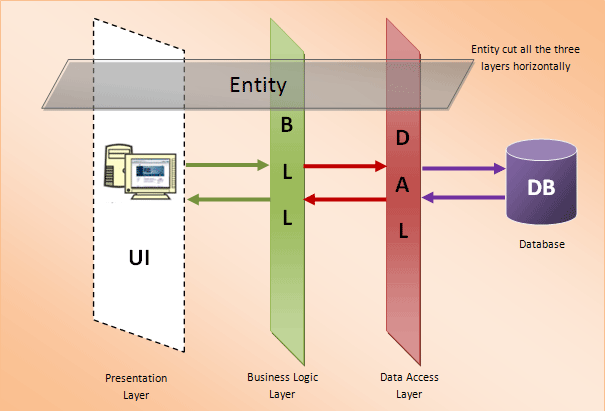
\includegraphics[width=\linewidth]{fig/3tier2}
	\caption{Concept of the 3-Tier Architectural pattern}
	\label{fig.setup}
\end{figure}
\noindent Analyzing the concept, we can see that it helps the application to
separate the \emph{input~logic}, \emph{business~logic} and \emph{UI~logic},
while providing a loose coupling between these elements. This allows for
independent development, testing and maintenance of each component - called
\emph{separation~of~concerns}.\\

\noindent Researching the frameworks that can help us carry out the current work,
we have found a few suitable candidates: \emph{Apache~Struts}, \emph{ASP.Net}
and \emph{Java~Server~Faces (JSF)}. When choosing the framework to use, we had
to take into consideration the following constraints:
\begin{itemize}
  \item the framework has to be free and open-source; free, because we do not
  have a budget to buy software and open-source because this is an academic
  project and should promote open-source
  \item we have an account on an ITU server to deploy the system; this
  server runs a Unix-like operating system; hence the framework should run on
  Unix-like platforms
\end{itemize}\\

\noindent \emph{ASP.Net} is a web application framework, developed by
Microsoft. We have excluded this candidate because it fails to adhere to both constraints
listed above; it is not open-source and runs only on the Microsoft Windows
platform.\\

\noindent \emph{Apache Struts} is an open-source web application framework
helping to develop Java EE web applications. It is based on the \emph{Java Servlet API},
encouraging the use of MVC architecture. This framework satisfies both
constraints, but it is a rather old technology, supporting
\emph{Java~Server~Pages (JSP)} for the presentation layer.\\

\noindent We wanted to go for something more fresh, choosing \emph{JSF~2}
as the framework to base our development upon. JSF is a Java-based web application
framework which simplifies the development integration of web-based user
interfaces. The core features, together with the help they offer for our
development process, are listed bellow, as summarized by \cite{wiki}. We have
leared the basics of JSF2 using \cite{Geary:3}.
\begin{itemize}
  \item managed beans (a \emph{dependency~injection} system) -- \emph{helps to
  easily manage the creation and injection of objects the system depends upon.}
  \item built in ajax support -- \emph{useful for dynamic form validations}
  \item integration with the \emph{Unified Expression Language (EL)}, which
  represent the core function of JSF; views may access managed bean fields and
  methods via EL
  \item a default set of HTML and web-application specific UI components -- to
  easily create good-looking and complex pages
  \item state management, supporting: ``request'', ``session'' and
  ``application''scoped Java beans -- \emph{helps to easily manage the lifetime
  of the managed beans}
\end{itemize}

\noindent A JSF application needs to be deployed in an environment that is
a \emph{web~server} and which provides a \emph{servlet~container}; although
there are many options (JBoss, Glassfish etc.) we chose the simplest,
\emph{Apache Tomcat 7}, which is a lightweight open source web server and
servlet container.\\

\noindent Moreover, to build a robust and safe system in
such a short period of time, we had to look for frameworks that can ease the development
process in the main areas of the project: presentation, business and data
access.

\paragraph{In the data access layer} the development can become a lot easier
having entities (classes) representing equivalents of the tables in the database. This
is an important aspect, as it is a lot easier to interact with the database in
an \emph{Object-Oriented (OO)} manner, from code written in an
OO language, by invoking operations on objects, then to write queries against
the database. For this purpose we chose \emph{Hibernate}, which is an 
\emph{object-relational mapping (ORM)} library for the Java language, providing
a framework for mapping an object-oriented domain model to a traditional
relational database.

\paragraph{In the business layer} the most important aspects are
\emph{security}, \emph{bean management} and \emph{flow~control}. We
immediately found a potential candidate which soon proved to be the a very good
one: the \emph{Spring Framework} - an open source application framework for the
Java platform, providing the following modules which we used:
\begin{itemize}
  \item \emph{Inversion of Control container (Dependency injection)} -
  container which provides a consistent means of configuring and managing Java
  objects using reflection. The container is responsible for managing
  object life-cycles: creating objects, calling initialization methods, and
  configuring objects by wiring them together \cite{wiki_spring}. Therefore, we
  used the bean manager provided by this module to manage JSF, Hibernate and
  Spring beans.
  \item \emph{Data access framework} (mostly in the data access layer) -
  addresses common difficulties developers face when working with databases in applications, providing support for all
  popular data access frameworks in Java (JDBC, Hibernate etc.). Some of the
  features made available by this module are: \emph{Resource
  management}\footnote{automatically acquiring and releasing database
  resources}, \emph{Exception handling}\footnote{translating data access related
  exception to a Spring data access hierarchy}, \emph{Transaction
  participation}\footnote{transparent participation in ongoing
  transactions},\emph{Resource unwrapping}\footnote{retrieving database objects
  from connection pool wrappers} \cite{wiki_spring}.
  \item \emph{Spring Security} - is a Java framework that provides
  \emph{authentication}, \emph{authorization} and other security features for
  enterprise applications.
\end{itemize}

\paragraph{In the presentation layer} in order to easily achieve a nice looking
user interface we used \emph{PrimeFaces}\footnote{http://www.primefaces.org/} - an open source
JSF component library featuring a large number of components. This is especially
good because we do not have any ``designer'' skills and using the components in
this library we had the chance to create a clean and ``shiny'' UI.\\

\noindent Summing up, our system is built upon \emph{JSF 2.1}, using
\emph{Hibernate 3.6} for ORM and \emph{Spring Framework 3} for bean management, data access and
security while using \emph{MySQL 5} for a database. The system is deployed in
\emph{Tomcat 7}. Combining these technologies was also enforced by
\emph{springsource} presentation \cite{tomcat_spring}, which states that Tomcat
and Spring are a perfect match.
